\section{Completed Capability Comparisons and Additional Controls}
\label{app:completed_results}

\subsection{Evaluation scope and the independent domain test}
\label{app:independent_domain_test}

Table~\ref{tab:completed_endpoints} reports ten joint-training configurations at update 500, each using training seed 42. This matrix combines the previously reported PG-DR and I64-DR/DT/GT Adam trajectories with I16-DR, PG-DT/GT Adam, and PG-DR/DT/GT SGD. It does not represent ten additional runs beyond the earlier trajectories. The original benchmarks contain 500 mathematics questions, a 128-question LiveCodeBench slice, 300 IFBench questions, and 198 GPQA-Diamond questions. Mathematics, code, and IF use one response per question; GPQA uses four responses, averaged within question. The full development grid comprises 37 trained checkpoints and one shared initial evaluation: updates 50/100/250/500 for the seven Adam trajectories and 100/250/500 for the three SGD trajectories.

Table~\ref{tab:independent_test} uses a separately frozen additional-domain test with 256 questions per domain, for 1,024 questions and 1,792 responses per model. Mathematics and code are drawn from the Skywork-OR1-RL-Data mathematics and TACO-based code pools; IF uses Nemotron-RL-instruction\_following; Science uses the Nemotron-RL-knowledge-mcqa validation split restricted by a fixed natural-science keyword filter. Questions are the first eligible unique candidates in frozen source order, selected without model scores. Normalized exact and lexical near-duplicate checks exclude the original training bundle and known evaluation pools. These checks do not establish exhaustive semantic decontamination or absence of pretraining exposure.

The additional test uses math answer verification, code unit tests, instruction-following constraints, and science multiple-choice scoring. Mathematics, code, and IF use greedy decoding; Science uses four responses per question at temperature 1. The generation context budget is 32,768 tokens, with thinking disabled. The source distributions and the code/IF scorers differ from the original benchmark protocol, so the two tables are reported separately. All completed code evaluations have zero recorded infrastructure errors. The four-domain mean is an equal-weight descriptive aggregate. The available question-paired bootstrap intervals describe finite-test uncertainty, not variability across independent training seeds.

% Generated by export.py from data.json; do not edit numbers.
\begin{table}[t]
\centering
\small
\setlength{\tabcolsep}{5pt}
\caption{Independent additional-domain test scores (percent). Each domain has 256 questions; Science averages four responses per question. This test uses different source distributions from the original benchmarks. Update 250 for PG-DT / Adam is included because both frozen selection rules chose it. All trained models use seed 42; Mean is the unweighted domain average.}
\label{tab:independent_test}
\begin{tabular}{lrrrrrr}
\toprule
Configuration & Update & Math & Code & IF & Science & Mean \\
\midrule
Initial student & 0 & 42.97 & 23.44 & 25.78 & 62.21 & 38.60 \\
PG-DR / Adam & 500 & 46.48 & 26.17 & 37.50 & 64.06 & 43.55 \\
PG-DT / Adam & 250 & 44.53 & 26.56 & 36.72 & 64.75 & 43.14 \\
PG-DT / Adam & 500 & 44.92 & 27.34 & 38.28 & 63.48 & 43.51 \\
PG-GT / Adam & 500 & 44.92 & 28.91 & 39.06 & 65.14 & 44.51 \\
I16-DR / Adam & 500 & 44.92 & 28.52 & 40.23 & 64.55 & 44.56 \\
I64-DR / Adam & 500 & 46.88 & 26.17 & 39.06 & 65.72 & 44.46 \\
I64-DT / Adam & 500 & 43.36 & 27.73 & 39.06 & 64.55 & 43.68 \\
I64-GT / Adam & 500 & 45.31 & 27.34 & 41.02 & 66.21 & 44.97 \\
PG-DR / SGD & 500 & 46.88 & 27.73 & 37.11 & 62.21 & 43.48 \\
PG-DT / SGD & 500 & 46.48 & 28.52 & 37.11 & 63.48 & 43.90 \\
PG-GT / SGD & 500 & 44.53 & 26.17 & 36.72 & 64.45 & 42.97 \\
\bottomrule
\end{tabular}
\end{table}


\subsection{Frozen checkpoint-selection outcomes}
\label{app:completed_selection}

The selection protocol fixes a tolerance of 2 percentage points per domain relative to initialization, equal domain weights, and a minimum useful mean gain of 1 percentage point. It compares the endpoint, maximum-development-utility checkpoint, and maximum-utility checkpoint satisfying the retention constraints. Selections were frozen before the selected models' independent test inference. Development selection uses the already observed original benchmarks and is therefore exploratory.

% Generated by export.py from data.json; do not edit numbers.
\begin{table}[t]
\centering
\small
\setlength{\tabcolsep}{5pt}
\caption{Frozen checkpoint choices. Max utility and retention select the same checkpoint in every trajectory. Test $\Delta$ is the selected-checkpoint mean minus the endpoint mean in percentage points.}
\label{tab:checkpoint_selection}
\begin{tabular}{lrrrr}
\toprule
Trajectory & Endpoint & Max utility & Retention & Test $\Delta$ (pp) \\
\midrule
Other nine trajectories & 500 & 500 & 500 & 0.000 \\
PG-DT / Adam & 500 & 250 & 250 & -0.366 \\
\bottomrule
\end{tabular}
\end{table}


The retention and maximum-utility rules select identical checkpoints in all ten trajectories. Nine trajectories select update 500 under all three rules. For PG-DT/Adam, the two selection rules choose update 250: its independent-test mean is 43.140\%, compared with 43.506\% at update 500. Thus this comparison does not establish an advantage for retention-constrained selection. All selected models satisfy the retention and useful-gain conditions as test point estimates; this is not a simultaneous confidence guarantee. PG-DR/Adam has two development checkpoints outside the tolerance: GPQA falls from 32.197\% initially to 28.030\% at update 50 and 30.177\% at update 250, before reaching 34.975\% at update 500. Endpoint retention therefore does not imply retention throughout training.

\subsection{Actual intersection coverage}
\label{app:actual_intersection_coverage}

% Generated by export.py from data.json; do not edit numbers.
\begin{table}[t]
\centering
\footnotesize
\setlength{\tabcolsep}{5pt}
\caption{I64 candidate intersections retain high student probability mass. Mass is in percent; means and minima are over sampled prefixes. $r=p_\theta(I\mid h)/p_\theta(S\mid h)$ is the retained weight ratio.}
\label{tab:intersection_coverage}
\begin{tabular}{lrrrrrr}
\toprule
Student state & $p(I)$: mean & $p(I)$: min & $|I|$: mean & $|I|$: min & $r$: mean & $r$: min \\
\midrule
M-PG/100 & 99.9141 & 96.5482 & 58.96 & 43 & 0.9999413 & 0.9977714 \\
M-PG/500 & 99.9952 & 99.7825 & 61.59 & 50 & 0.9999975 & 0.9998511 \\
M-I64-DR/100 & 99.9564 & 97.5664 & 60.08 & 36 & 0.9997331 & 0.9757993 \\
M-I64-DR/500 & 99.9826 & 99.3722 & 61.75 & 51 & 0.9999912 & 0.9997005 \\
\bottomrule
\end{tabular}
\end{table}


Table~\ref{tab:intersection_coverage} measures the student probability mass in the actual student--teacher candidate intersection, rather than in the teacher candidate set alone. All 384 sampled routed prefixes have intersection mass above 95\%, and none has an empty intersection. This high-coverage regime helps delimit the local comparisons with full-vocabulary feedback. It does not establish the same behavior for low-coverage prefixes, other teacher configurations, or the full online I16 training trajectory. The four banks are local sampling repeats, not independent training seeds; inputs can differ across student states.

\subsection{Sensitivity to known mathematics overlap}
\label{app:math_overlap_sensitivity}

The frozen Qwen training pool contains five records matching four known MATH-500 underlying problems, including wording or answer-form variants. The affected MATH test identifiers are counting-and-probability problem 430 and intermediate-algebra problems 1849, 2146, and 582. Their presence in the training pool does not establish that each was sampled by a particular run or caused a performance increase. We remove these four fixed evaluation questions from the existing per-question scores as an offline sensitivity analysis, retaining the original 500-question results as the main protocol.

% MATH subset scores retained; means synchronized with the authoritative Table 1 domain scores.
\begin{table}[t]
\centering
\small
\setlength{\tabcolsep}{5pt}
\caption{\textbf{Removing four overlapping mathematics questions can reorder near-tied configurations.} Mean (496) substitutes MATH-496 for MATH-500 and keeps the other domain scores fixed.}
\label{tab:math496_sensitivity}
\begin{tabular}{lrrrrr}
\toprule
Configuration & Update & MATH-500 & MATH-496 & Mean (500) & Mean (496) \\
\midrule
Initial student & 0 & 68.80 & 69.15 & 33.94 & 34.02 \\
PG-DR / Adam & 500 & 73.20 & 73.79 & 38.61 & 38.76 \\
PG-DT / Adam & 250 & 77.00 & 77.42 & 38.78 & 38.89 \\
PG-DT / Adam & 500 & 73.20 & 73.59 & 38.60 & 38.70 \\
PG-GT / Adam & 500 & 76.20 & 76.81 & 38.60 & 38.75 \\
I16-DR / Adam & 500 & 75.40 & 76.01 & 38.90 & 39.06 \\
I64-DR / Adam & 500 & 75.80 & 76.41 & 39.04 & 39.19 \\
I64-DT / Adam & 500 & 74.00 & 74.40 & 39.19 & 39.29 \\
I64-GT / Adam & 500 & 74.20 & 74.60 & 39.02 & 39.12 \\
PG-DR / SGD & 500 & 76.40 & 77.02 & 39.96 & 40.12 \\
PG-DT / SGD & 500 & 75.20 & 75.81 & 39.44 & 39.59 \\
PG-GT / SGD & 500 & 75.00 & 75.60 & 38.58 & 38.73 \\
\bottomrule
\end{tabular}
\end{table}


The ordering by four-domain mean is unchanged across the twelve reported checkpoints. The frozen checkpoint selections are retained. This comparison neither retrains on a filtered pool nor constitutes an exhaustive overlap or contamination audit.

\subsection{Teacher-update overlap and distributional similarity}
\label{app:teacher_overlap_support}

\begin{figure}[t]
\centering
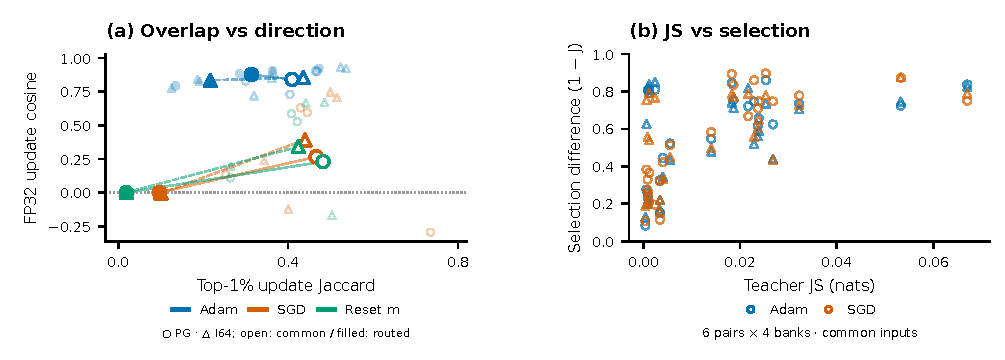
\includegraphics[width=\linewidth]{figures/nine_panel_20260914/appendix_teacher_overlap.pdf}
\caption{Supporting overlap views at the shared M-PG/500 student and optimizer state. (a) Top-1\% FP32 update-set Jaccard versus update cosine for PG/I64, common/routed inputs, and saved-state Adam, reset-$m$, and norm-matched SGD. Small points summarize banks and large points average four banks. (b) Common-input teacher JS versus $1-$Jaccard for Adam and SGD; each point is one teacher pair within one bank (six pairs per bank, four banks). Pairs share teachers and banks, so these points are dependent. These geometric associations do not measure cross-domain capability harm.}
\label{fig:teacher_overlap_support}
\end{figure}

Figure~\ref{fig:teacher_overlap_support} preserves the overlap and teacher-distribution comparisons alongside the history-subtracted controls in the main text. It uses local updates on copies of a saved state, not bitwise replay of the online optimizer. Common inputs hold the student prefixes fixed across teachers; routed inputs change the teacher and its input domain together.
